% Source-backed analysis update assembled from:
%   ../docs/ml_results.md
%   ../docs/progress.md
%   ../docs/roadmap.md
%   ../Analysis_CODES/docs/ppref_x_reweighted_working_points.md
%   ../Analysis_CODES/docs/pbpb24_psi2s_selection_mass_scan.md
\documentclass[11pt,aspectratio=169]{beamer}

\usetheme{Madrid}
\usecolortheme{default}
\setbeamertemplate{navigation symbols}{}
\setbeamertemplate{footline}[frame number]

\usepackage{booktabs}
\usepackage{graphicx}
\usepackage{tikz}
\usetikzlibrary{arrows.meta,positioning}
\input{beamer_setup.tex}

\definecolor{positive}{HTML}{0173B2}
\definecolor{negative}{HTML}{DE8F05}
\definecolor{emphasis}{HTML}{027A5A}
\definecolor{neutral}{HTML}{666666}
\definecolor{panelbg}{HTML}{F4F6F8}
\setbeamercolor{structure}{fg=positive}
\setbeamercolor{block title}{fg=white,bg=positive}
\setbeamercolor{block body}{fg=black,bg=positive!8}
\setbeamercolor{block title alerted}{fg=white,bg=negative}
\setbeamercolor{block body alerted}{fg=black,bg=negative!10}
\setbeamercolor{block title example}{fg=white,bg=emphasis}
\setbeamercolor{block body example}{fg=black,bg=emphasis!8}
\newcommand{\pos}[1]{\textcolor{positive}{#1}}
\newcommand{\con}[1]{\textcolor{negative}{#1}}
\newcommand{\HL}[1]{\textcolor{emphasis}{#1}}
\newcommand{\muted}[1]{\textcolor{neutral}{#1}}

\title[X(3872) Analysis Update]{X(3872) Analysis Update}
\subtitle{From \texorpdfstring{\psiP}{psi(2S)} reweighting to the current PbPb strategy}
\author{Lekai Yao}
\institute{CMS}
\date{2026.7.29}

\begin{document}

\begin{frame}[plain]
  \titlepage
  \vspace{-0.6em}
  \begin{center}
    \small ppRef prototype completed --- PbPb selection and fit diagnostics in progress
  \end{center}
\end{frame}

\begin{frame}{Why can MC mismodelling bias the X analysis?}
  \begin{columns}[T]
    \begin{column}{0.46\textwidth}
      \centering
      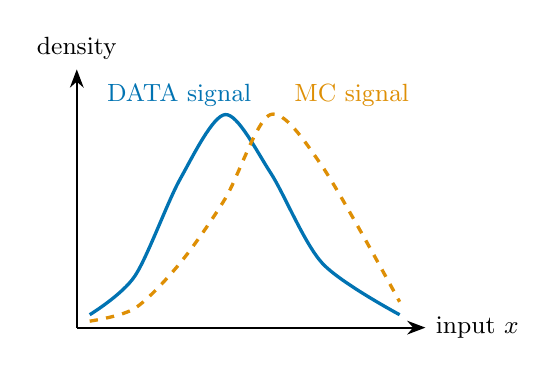
\begin{tikzpicture}[
        x=0.82cm,y=0.82cm,
        axis/.style={-{Stealth},thick},
        data/.style={positive,very thick},
        mc/.style={negative,very thick,dashed}
      ]
        \draw[axis] (0,0) -- (5.4,0) node[right] {\small input $x$};
        \draw[axis] (0,0) -- (0,4.0) node[above] {\small density};
        \draw[data] plot[smooth] coordinates
          {(0.2,0.2) (0.9,0.8) (1.6,2.3) (2.3,3.3)
           (3.0,2.4) (3.8,1.0) (5.0,0.2)};
        \draw[mc] plot[smooth] coordinates
          {(0.2,0.1) (0.9,0.3) (1.6,1.0) (2.3,2.0)
           (3.0,3.3) (3.8,2.5) (5.0,0.4)};
        \node[data,anchor=west] at (0.3,3.6) {\small DATA signal};
        \node[mc,anchor=west] at (3.2,3.6) {\small MC signal};
      \end{tikzpicture}
      \vspace{0.4em}

      \small The classifier sees the simulated signal distribution,
      not the unknown true X signal distribution.
    \end{column}
    \begin{column}{0.51\textwidth}
      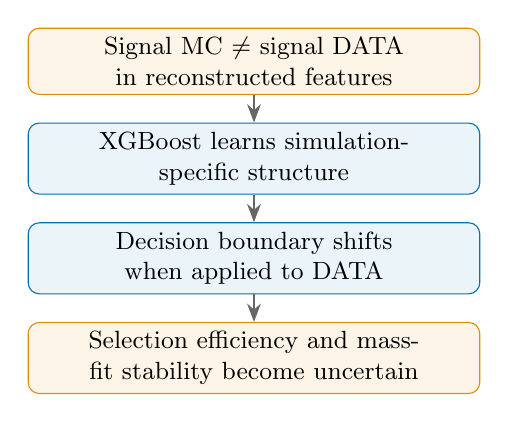
\begin{tikzpicture}[
        node distance=0.35cm,
        box/.style={
          draw=positive,
          rounded corners,
          fill=positive!8,
          text width=5.5cm,
          minimum height=0.75cm,
          align=center,
          font=\small
        },
        warn/.style={
          draw=negative,
          rounded corners,
          fill=negative!10,
          text width=5.5cm,
          minimum height=0.75cm,
          align=center,
          font=\small
        },
        arr/.style={-{Stealth},thick,neutral}
      ]
        \node[warn] (mismatch) {Signal MC $\neq$ signal DATA in reconstructed features};
        \node[box,below=of mismatch] (learn) {XGBoost learns simulation-specific structure};
        \node[box,below=of learn] (shift) {Decision boundary shifts when applied to DATA};
        \node[warn,below=of shift] (eff) {Selection efficiency and mass-fit stability become uncertain};
        \draw[arr] (mismatch) -- (learn);
        \draw[arr] (learn) -- (shift);
        \draw[arr] (shift) -- (eff);
      \end{tikzpicture}
    \end{column}
  \end{columns}
  \vfill
  \centering\HL{A more powerful classifier does not by itself remove a domain mismatch.}
\end{frame}

\begin{frame}{Event reweighting as multidimensional density-ratio estimation}
  \begin{columns}[T]
    \begin{column}{0.48\textwidth}
      \begin{block}{Target correction}
        \[
          w(\mathbf{x})
          \simeq
          \frac{p_{\mathrm{DATA\ signal}}(\mathbf{x})}
               {p_{\mathrm{MC\ signal}}(\mathbf{x})}.
        \]
      \end{block}
      \[
        p_{\mathrm{MC}}^{\mathrm{weighted}}(\mathbf{x})
        \approx p_{\mathrm{DATA\ signal}}(\mathbf{x}).
      \]
    \end{column}
    \begin{column}{0.48\textwidth}
      \begin{itemize}
        \item $\mathbf{x}$: correlated reconstruction-level variables
        \item One continuous weight per simulated event
        \item BDT reweighter handles the multidimensional ratio
        \item No event reconstruction is changed
        \item No new simulated events are created
      \end{itemize}
    \end{column}
  \end{columns}
  \vspace{0.5em}
  \centering
  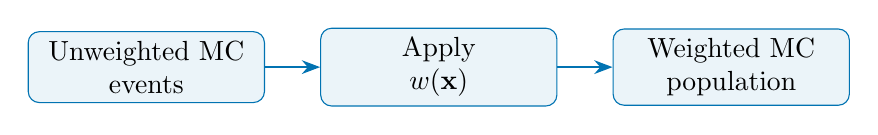
\begin{tikzpicture}[
    node distance=0.7cm,
    box/.style={
      draw=positive,
      rounded corners,
      fill=positive!8,
      minimum width=3.0cm,
      minimum height=0.9cm,
      align=center
    },
    arr/.style={-{Stealth},thick,positive}
  ]
    \node[box] (mc) {Unweighted MC\\events};
    \node[box,right=of mc] (weight) {Apply\\$w(\mathbf{x})$};
    \node[box,right=of weight] (weighted) {Weighted MC\\population};
    \draw[arr] (mc) -- (weight);
    \draw[arr] (weight) -- (weighted);
  \end{tikzpicture}
  \vfill
  \centering\small
  BDT reweighting: A. Rogozhnikov, arXiv:1608.05806.
\end{frame}

\begin{frame}{The DATA target must represent signal, not inclusive background}
  \begin{columns}[T]
    \begin{column}{0.48\textwidth}
      \centering
      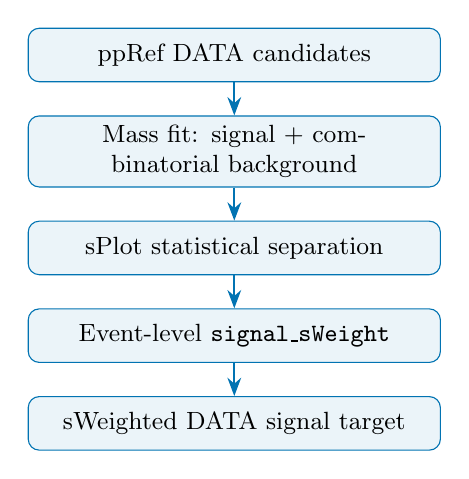
\begin{tikzpicture}[
        node distance=0.42cm,
        box/.style={
          draw=positive,
          rounded corners,
          fill=positive!8,
          text width=5.0cm,
          minimum height=0.68cm,
          align=center,
          font=\small
        },
        arr/.style={-{Stealth},thick,positive}
      ]
        \node[box] (cand) {ppRef \psiP DATA candidates};
        \node[box,below=of cand] (fit) {Mass fit: signal + combinatorial background};
        \node[box,below=of fit] (splot) {sPlot statistical separation};
        \node[box,below=of splot] (tree) {Event-level \texttt{signal\_sWeight}};
        \node[box,below=of tree] (target) {sWeighted DATA signal target};
        \draw[arr] (cand) -- (fit);
        \draw[arr] (fit) -- (splot);
        \draw[arr] (splot) -- (tree);
        \draw[arr] (tree) -- (target);
      \end{tikzpicture}
    \end{column}
    \begin{column}{0.48\textwidth}
      \begin{block}{What the target is}
        \begin{itemize}
          \item Statistical representation of the signal component
          \item Negative sWeights retained
          \item Fit and effective-statistics diagnostics required
        \end{itemize}
      \end{block}
      \begin{alertblock}{What it is not}
        \begin{itemize}
          \item Not an event-by-event truth label
          \item Not equivalent to a pure simulated signal sample
          \item Not usable without a trustworthy mass fit
        \end{itemize}
      \end{alertblock}
    \end{column}
  \end{columns}
\end{frame}

\begin{frame}{What is transferred from \texorpdfstring{\psiP}{psi(2S)} to X?}
  \begin{columns}[T]
    \begin{column}{0.48\textwidth}
      \begin{exampleblock}{Transfer}
        \begin{itemize}
          \item DATA/MC correction in shared variables
          \item Tracking and vertex reconstruction response
          \item Correction inside validated phase-space support
          \item Event weights applied to X simulation
        \end{itemize}
      \end{exampleblock}
    \end{column}
    \begin{column}{0.48\textwidth}
      \begin{alertblock}{Do not transfer}
        \begin{itemize}
          \item Raw \psiP physics distribution
          \item \psiP mass or dipion dynamics
          \item A \psiP-trained classifier
          \item Unconstrained correction outside target support
        \end{itemize}
      \end{alertblock}
    \end{column}
  \end{columns}
  \vspace{0.7em}
  \begin{block}{Transfer assumption to validate}
    \[
      \left[\frac{p_{\mathrm{DATA}}}{p_{\mathrm{MC}}}\right]_{\psiP}
      (\mathbf{x}\mid\mathbf{z})
      \approx
      \left[\frac{p_{\mathrm{DATA}}}{p_{\mathrm{MC}}}\right]_{X}
      (\mathbf{x}\mid\mathbf{z}),
    \]
  \end{block}
  \centering\small
  $\mathbf{x}$: shared detector/reconstruction variables;\quad
  $\mathbf{z}$: conditioning kinematics such as $p_{\mathrm{T}}$ and rapidity.
\end{frame}

\begin{frame}{Analysis path: validate the chain, then move to PbPb}
  \centering
  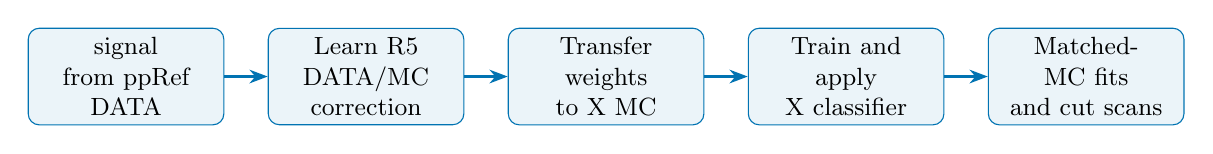
\begin{tikzpicture}[
    node distance=0.55cm,
    box/.style={
      draw=positive,
      rounded corners,
      fill=positive!8,
      minimum height=0.82cm,
      text width=2.25cm,
      align=center,
      font=\small
    },
    arrow/.style={-{Stealth},thick,positive}
  ]
    \node[box] (signal) {\psiP signal\\from ppRef DATA};
    \node[box,right=of signal] (rw) {Learn R5\\DATA/MC correction};
    \node[box,right=of rw] (apply) {Transfer weights\\to X MC};
    \node[box,right=of apply] (ml) {Train and apply\\X classifier};
    \node[box,right=of ml] (fit) {Matched-MC fits\\and cut scans};
    \draw[arrow] (signal) -- (rw);
    \draw[arrow] (rw) -- (apply);
    \draw[arrow] (apply) -- (ml);
    \draw[arrow] (ml) -- (fit);
  \end{tikzpicture}

  \vspace{1.0em}
  \begin{columns}[T]
    \begin{column}{0.48\textwidth}
      \begin{block}{ppRef question}
        Can the complete correction $\rightarrow$ ML $\rightarrow$ fit workflow be validated?
      \end{block}
    \end{column}
    \begin{column}{0.48\textwidth}
      \begin{alertblock}{Interpretation boundary}
        Observed significance alone does not establish the final training preference.
      \end{alertblock}
    \end{column}
  \end{columns}
  \vfill
  \centering\small\HL{The ppRef prototype is now closed; the next bottleneck is PbPb \psiP.}
\end{frame}

\begin{frame}{Reweighting profiles: variable definitions}
  \vspace{4pt}
  \begin{center}
    \small
    \begin{tabular}{lp{9.7cm}}
      \toprule
      Profile & Reweighting variables \\
      \midrule
      R3 &
      \texttt{Bcos\_dtheta}, \texttt{Btktkpt}, \texttt{Bchi2Prob} \\
      \addlinespace
      R4-noCos &
      \texttt{Btktkpt}, \texttt{Bchi2Prob},
      \texttt{Btrk1Pt}, \texttt{Btrk2Pt} \\
      \addlinespace
      R5 &
      \texttt{Bcos\_dtheta}, \texttt{Btktkpt}, \texttt{Bchi2Prob},
      \texttt{Btrk1Pt}, \texttt{Btrk2Pt} \\
      \addlinespace
      R8 &
      \texttt{Bchi2Prob}, \texttt{Btrk1dR}, \texttt{BtrkPtimb},
      \texttt{Btrk1Pt}, \texttt{Btrk2Pt}, \texttt{BtktkvProb},
      \texttt{Bcos\_dtheta}, \texttt{Btktkpt} \\
      \bottomrule
    \end{tabular}
  \end{center}
  \vspace{0.4em}
  \begin{columns}[T]
    \begin{column}{0.48\textwidth}
      \begin{block}{Controlled comparisons}
        R3: low-dimensional check;\quad
        R4-noCos: remove \texttt{Bcos\_dtheta}.
      \end{block}
    \end{column}
    \begin{column}{0.48\textwidth}
      \begin{exampleblock}{Prototype decision}
        R5 nominal;\quad R8 excluded because of weight tails and loss of effective statistics.
      \end{exampleblock}
    \end{column}
  \end{columns}
\end{frame}

\begin{frame}{Reweighting profiles: KS-like closure metric}
  \begin{columns}[T]
    \begin{column}{0.52\textwidth}
      \vspace{4pt}
      \begin{center}
        \small
        \begin{tabular}{lrr}
          \toprule
          Profile & Mean before & Mean after \\
          \midrule
          R3       & 0.0908 & 0.0100 \\
          R4-noCos & 0.0908 & 0.0409 \\
          R5       & 0.0908 & \textbf{0.0091} \\
          R8       & 0.0908 & 0.0123 \\
          \bottomrule
        \end{tabular}
      \end{center}
      \vspace{0.5em}
      \begin{alertblock}{Metric interpretation}
        \small Mean maximum CDF distance over eight validation variables,
        using signed target weights. Descriptive KS-like distance, not a KS p-value.
      \end{alertblock}
    \end{column}
    \begin{column}{0.45\textwidth}
      \centering
      \includegraphics[width=\textwidth,height=0.65\textheight,keepaspectratio]
      {../XGBoost/output/reweighting/comparison_pp24_psi2s/weight_distributions_R3_R4_R5_R8.pdf}
    \end{column}
  \end{columns}
  \vfill
  \centering\small
  R5 gives the best average one-dimensional closure without the R8 weight instability.
\end{frame}

\begin{frame}{One-dimensional closure: before and after R5}
  \begin{columns}[T]
    \begin{column}{0.49\textwidth}
      \centering
      \textbf{\texttt{Bcos\_dtheta}}\\[-0.2em]
      \includegraphics[width=\textwidth,height=0.66\textheight,keepaspectratio]
      {../XGBoost/output/reweighting/comparison_pp24_psi2s/variable_closure/Bcos_dtheta_before_after_ratio.pdf}
    \end{column}
    \begin{column}{0.49\textwidth}
      \centering
      \textbf{\texttt{Bchi2Prob}}\\[-0.2em]
      \includegraphics[width=\textwidth,height=0.66\textheight,keepaspectratio]
      {../XGBoost/output/reweighting/comparison_pp24_psi2s/variable_closure/Bchi2Prob_before_after_ratio.pdf}
    \end{column}
  \end{columns}
  \vfill
  \centering\small
  One-dimensional agreement is necessary, but correlations require an independent multivariate test.
\end{frame}

\begin{frame}{Closure: little residual DATA/MC separation}
  \begin{columns}[T]
    \begin{column}{0.52\textwidth}
      \centering
      \includegraphics[width=\textwidth,height=0.60\textheight,keepaspectratio]
      {../XGBoost/output/reweighting/comparison_pp24_psi2s/domain_auc_stability.pdf}
    \end{column}
    \begin{column}{0.45\textwidth}
      \begin{exampleblock}{Independent holdout test}
        Domain-classifier AUC $\simeq \HL{0.5225}$, stable over five random splits.
      \end{exampleblock}
      \begin{itemize}
        \item Weight statistics validated
        \item X MC support/coverage checked
        \item \texttt{Reweight} written to X MC
        \item No obvious residual separation
      \end{itemize}
    \end{column}
  \end{columns}
  \vfill
  \centering\small\HL{R5 passes the ppRef closure and transfer checks used in this prototype.}
\end{frame}

\begin{frame}{X classifier: unweighted and R5-weighted 8v2}
  \begin{columns}[T]
    \begin{column}{0.49\textwidth}
      \centering
      \textbf{Unweighted X MC}\\[-0.1em]
      \includegraphics[width=\textwidth,height=0.58\textheight,keepaspectratio]
      {../XGBoost/output/training/X_pp24_v4_fid3_8v2_rw0_xgb_v1/roc.pdf}
      \scriptsize
      \texttt{X\_pp24\_v4\_fid3\_8v2\_rw0\_xgb\_v1}
    \end{column}
    \begin{column}{0.49\textwidth}
      \centering
      \textbf{R5-weighted X MC}\\[-0.1em]
      \includegraphics[width=\textwidth,height=0.58\textheight,keepaspectratio]
      {../XGBoost/output/training/X_pp24_v4_fid3_8v2_rwpsi2sr5v1_xgb_v1/roc.pdf}
      \scriptsize
      \texttt{X\_pp24\_v4\_fid3\_8v2\_rwpsi2sr5v1\_xgb\_v1}
    \end{column}
  \end{columns}
  \vfill
  \centering\small
  Both train/apply/draw chains and scored DATA/MC ROOT files are complete.
\end{frame}

\begin{frame}{Matched-MC working points}
  \vspace{4pt}
  \begin{center}
    \small
    \begin{tabular}{llrrrr}
      \toprule
      Training & Bkg. eff. & Status & Yield & Signif. & Mass [GeV] \\
      \midrule
      rw0 & 10\% & 0/0 & $762\pm63$ & 12.18 & 3.87028 \\
      rw0 & 3\%  & $-1$/3 & $286\pm80$ & 8.04 & 3.86884 \\
      rw0 & 1\%  & 0/0 & $112\pm20$ & 5.52 & 3.86703 \\
      \midrule
      R5 & 10\% & 0/0 & $775\pm65$ & 12.21 & 3.87174 \\
      R5 & 3\%  & 0/0 & $216\pm54$ & 5.84 & 3.87229 \\
      R5 & 1\%  & 0/0 & $78\pm23$ & 3.40 & 3.87208 \\
      \bottomrule
    \end{tabular}
  \end{center}
  \vspace{0.3em}
  \begin{columns}[T]
    \begin{column}{0.48\textwidth}
      \begin{block}{Interface fixed}
        Each training uses its own scored DATA and matched MC template.
      \end{block}
    \end{column}
    \begin{column}{0.48\textwidth}
      \begin{alertblock}{Comparison caveat}
        rw0 3\% did not converge; it cannot support a quantitative ranking.
      \end{alertblock}
    \end{column}
  \end{columns}
  \vfill
  \centering\small
  No consistent R5 sensitivity gain across the three predefined working points.
\end{frame}

\begin{frame}{Punzi optimum: useful diagnostic, not a final ranking}
  \vspace{4pt}
  \begin{center}
    \begin{tabular}{lrrrr}
      \toprule
      Training & Frozen cut & Efficiency & Fit status & Significance \\
      \midrule
      rw0 & 0.875 & 0.2840 & strategy-2: 0/0 & 7.01 \\
      R5  & 0.613 & 0.6775 & 0/0 & 16.62 \\
      \bottomrule
    \end{tabular}
  \end{center}
  \vspace{0.8em}
  \begin{columns}[T]
    \begin{column}{0.48\textwidth}
      \begin{block}{What was validated}
        \begin{itemize}
          \item Frozen before inspecting new fits
          \item R5 fit converges with a clear X peak
          \item R5 cut agrees with the later 0.6 scan point
        \end{itemize}
      \end{block}
    \end{column}
    \begin{column}{0.48\textwidth}
      \begin{alertblock}{Why this is not the answer}
        \begin{itemize}
          \item Efficiency definitions differ
          \item rw0 cut 0.875 is too tight in DATA
          \item Significance cannot rank the schemes alone
        \end{itemize}
      \end{alertblock}
    \end{column}
  \end{columns}
\end{frame}

\begin{frame}{Fixed-cut scans expose the relevant trend}
  \vspace{4pt}
  \begin{center}
    \small
    \begin{tabular}{lrrr}
      \toprule
      Scan & Prediction range & Significance trend & Fitted mass range [GeV] \\
      \midrule
      rw0 & 0.2--0.8 & $20.27 \rightarrow 9.49$ & $3.87128 \rightarrow 3.86914$ \\
      R5  & 0.2--0.8 & $\sim20 \rightarrow 6.63$ & $3.87113$--$3.87204$ \\
      \bottomrule
    \end{tabular}
  \end{center}
  \vspace{0.6em}
  \begin{columns}[T]
    \begin{column}{0.48\textwidth}
      \begin{block}{rw0}
        \begin{itemize}
          \item Seven default fits converge
          \item Yield/significance fall with tighter cuts
          \item Frozen 0.875 is beyond the useful scan
        \end{itemize}
      \end{block}
    \end{column}
    \begin{column}{0.48\textwidth}
      \begin{exampleblock}{R5}
        \begin{itemize}
          \item More stable fitted peak position
          \item Cut 0.8 passes strategy-2 check
          \item $S(0.613)=16.62$, $S(0.6)=16.91$
        \end{itemize}
      \end{exampleblock}
    \end{column}
  \end{columns}
  \vfill
  \centering\small
  \HL{ppRef validates the chain, but does not uniquely choose the final correction scheme.}
\end{frame}

\begin{frame}{PbPb \texorpdfstring{\psiP}{psi(2S)}: cumulative S0--S4 definitions}
  \vspace{4pt}
  \begin{center}
    \small
    \begin{tabular}{lp{10.5cm}}
      \toprule
      ID & Selection \\
      \midrule
      S0 &
      \texttt{BQvalue < 0.15 \&\& abs(By) < 1.6 \&\& Bpt > 10} \\
      \addlinespace
      S1 &
      S0, but tighten \texttt{abs(By) < 1.2} \\
      \addlinespace
      S2 &
      S1 \texttt{\&\& Btrk2dR < 0.25} \\
      \addlinespace
      S3 &
      S2 \texttt{\&\& BtrkPtimb > 0.15} \\
      \addlinespace
      S4 &
      S3 \texttt{\&\& Btrk1dR < 0.25} \\
      \bottomrule
    \end{tabular}
  \end{center}
  \vspace{0.6em}
  \begin{columns}[T]
    \begin{column}{0.48\textwidth}
      \begin{block}{Design}
        \begin{itemize}
          \item Same $3.6<m<3.8$ GeV range
          \item Same 5 MeV binning
          \item Strictly cumulative selections
        \end{itemize}
      \end{block}
    \end{column}
    \begin{column}{0.48\textwidth}
      \begin{alertblock}{ML interaction}
        \begin{itemize}
          \item \texttt{Btrk2dR}: not planned for R5 ML
          \item \texttt{BtrkPtimb}, \texttt{Btrk1dR}: ML candidates
          \item S3/S4 are diagnostic, not nominal
        \end{itemize}
      \end{alertblock}
    \end{column}
  \end{columns}
\end{frame}

\begin{frame}{PbPb \texorpdfstring{\psiP}{psi(2S)} mass spectra: S0 and S1}
  \begin{columns}[T]
    \begin{column}{0.49\textwidth}
      \centering
      \textbf{S0 --- common fiducial baseline}\\[-0.2em]
      \includegraphics[width=\textwidth,height=0.69\textheight,keepaspectratio]
      {../Analysis_CODES/plotER/results/PbPb24/psi2s_selection_mass_scan/PbPb24_psi2S_S0_3p6_3p8.pdf}
      \small 497,145 entries in $3.6<m<3.8$ GeV
    \end{column}
    \begin{column}{0.49\textwidth}
      \centering
      \textbf{S1 --- tighter rapidity}\\[-0.2em]
      \includegraphics[width=\textwidth,height=0.69\textheight,keepaspectratio]
      {../Analysis_CODES/plotER/results/PbPb24/psi2s_selection_mass_scan/PbPb24_psi2S_S1_3p6_3p8.pdf}
      \small 373,736 entries in $3.6<m<3.8$ GeV
    \end{column}
  \end{columns}
\end{frame}

\begin{frame}{PbPb \texorpdfstring{\psiP}{psi(2S)} mass spectra: S2 and S3}
  \begin{columns}[T]
    \begin{column}{0.49\textwidth}
      \centering
      \textbf{S2 --- add \texttt{Btrk2dR < 0.25}}\\[-0.2em]
      \includegraphics[width=\textwidth,height=0.69\textheight,keepaspectratio]
      {../Analysis_CODES/plotER/results/PbPb24/psi2s_selection_mass_scan/PbPb24_psi2S_S2_3p6_3p8.pdf}
      \small 230,447 entries; preferred fit candidate
    \end{column}
    \begin{column}{0.49\textwidth}
      \centering
      \textbf{S3 --- add \texttt{BtrkPtimb > 0.15}}\\[-0.2em]
      \includegraphics[width=\textwidth,height=0.69\textheight,keepaspectratio]
      {../Analysis_CODES/plotER/results/PbPb24/psi2s_selection_mass_scan/PbPb24_psi2S_S3_3p6_3p8.pdf}
      \small 83,754 entries; tighter fallback
    \end{column}
  \end{columns}
\end{frame}

\begin{frame}{PbPb \texorpdfstring{\psiP}{psi(2S)} mass spectrum: S4}
  \begin{columns}[T]
    \begin{column}{0.64\textwidth}
      \centering
      \includegraphics[width=\textwidth,height=0.72\textheight,keepaspectratio]
      {../Analysis_CODES/plotER/results/PbPb24/psi2s_selection_mass_scan/PbPb24_psi2S_S4_3p6_3p8.pdf}
    \end{column}
    \begin{column}{0.33\textwidth}
      \begin{block}{S4: strict diagnostic point}
        \begin{itemize}
          \item Add \texttt{Btrk1dR < 0.25}
          \item 52,479 entries in the main window
          \item Cuts two ML-candidate variables
        \end{itemize}
      \end{block}
      \begin{alertblock}{Decision}
        S2 and S3, not S4, were retained for the consistent preliminary fits.
      \end{alertblock}
    \end{column}
  \end{columns}
\end{frame}

\begin{frame}{Current checkpoint: preliminary PbPb S2/S3 fits}
  \begin{columns}[T]
    \begin{column}{0.49\textwidth}
      \centering
      \textbf{S2 --- preferred candidate}\\[-0.2em]
      \includegraphics[width=\textwidth,height=0.42\textheight,keepaspectratio]
      {../Analysis_CODES/fitER/results/PbPb_H004_fit2_S2/data_fit_clean.pdf}
      \small
      \[
        N_{\psiP}=651\pm192,\quad
        \frac{S}{\sqrt{S+B}}=4.39
      \]
    \end{column}
    \begin{column}{0.49\textwidth}
      \centering
      \textbf{S3 --- tighter fallback}\\[-0.2em]
      \includegraphics[width=\textwidth,height=0.42\textheight,keepaspectratio]
      {../Analysis_CODES/fitER/results/PbPb_H004_fit2_S3/data_fit_clean.pdf}
      \small
      \[
        N_{\psiP}=301\pm113,\quad
        \frac{S}{\sqrt{S+B}}=3.41
      \]
    \end{column}
  \end{columns}
  \vspace{0.2em}
  \begin{alertblock}{Fit diagnostics in progress}
    \small Both fits have status/covQual $=0/3$; the DATA width scale reaches 1.15.
    Results are preliminary; sWeight and $N_{\mathrm{eff}}$ checks are pending.
  \end{alertblock}
\end{frame}

\begin{frame}{Status and immediate next steps}
  \begin{columns}[T]
    \begin{column}{0.48\textwidth}
      \begin{exampleblock}{Completed: ppRef prototype}
        \begin{itemize}
          \item \psiP signal target and R5 correction
          \item Closure and transfer to X MC
          \item rw0/R5 train, apply, matched fits
          \item Prediction scans and physical review
        \end{itemize}
      \end{exampleblock}
    \end{column}
    \begin{column}{0.48\textwidth}
      \begin{block}{Next: PbPb-specific chain}
        \begin{enumerate}
          \item Accept S2 or S3 fit configuration
          \item Produce and validate sWeights
          \item Train PbPb-specific correction
          \item Retrain X ML and scan Prediction
        \end{enumerate}
      \end{block}
    \end{column}
  \end{columns}
  \vfill
  \begin{center}
    \Large\HL{The ppRef chain is validated.}\\[0.4em]
    \normalsize
    The immediate decision is whether the preliminary PbPb \psiP fit is robust enough
    to provide the next reweighting target.
  \end{center}
\end{frame}

\appendix

\begin{frame}{Backup: additional R5 variable closure}
  \begin{columns}[T]
    \begin{column}{0.49\textwidth}
      \centering
      \includegraphics[width=\textwidth,height=0.37\textheight,keepaspectratio]
      {../XGBoost/output/reweighting/comparison_pp24_psi2s/variable_closure/Btktkpt_before_after_ratio.pdf}

      \includegraphics[width=\textwidth,height=0.37\textheight,keepaspectratio]
      {../XGBoost/output/reweighting/comparison_pp24_psi2s/variable_closure/Btrk1Pt_before_after_ratio.pdf}
    \end{column}
    \begin{column}{0.49\textwidth}
      \centering
      \includegraphics[width=\textwidth,height=0.37\textheight,keepaspectratio]
      {../XGBoost/output/reweighting/comparison_pp24_psi2s/variable_closure/Btrk2Pt_before_after_ratio.pdf}

      \includegraphics[width=\textwidth,height=0.37\textheight,keepaspectratio]
      {../XGBoost/output/reweighting/comparison_pp24_psi2s/variable_closure/BtrkPtimb_before_after_ratio.pdf}
    \end{column}
  \end{columns}
\end{frame}

\begin{frame}{Backup: rw0 fixed-cut scan}
  \vspace{4pt}
  \begin{center}
    \small
    \begin{tabular}{rrrrrrr}
      \toprule
      Cut & DATA & MC & Status & Yield & Signif. & Mass [GeV] \\
      \midrule
      0.2 & 104673 & 82611 & 0/0 & $2995\pm156$ & 20.27 & 3.87128 \\
      0.3 & 84800  & 79852 & 0/0 & $2596\pm168$ & 19.56 & 3.87098 \\
      0.4 & 67465  & 76051 & 0/0 & $2045\pm156$ & 18.15 & 3.87075 \\
      0.5 & 51473  & 70655 & 0/0 & $1647\pm133$ & 16.98 & 3.87069 \\
      0.6 & 35775  & 62777 & 0/0 & $1141\pm88$  & 14.56 & 3.87040 \\
      0.7 & 22553  & 52784 & 0/0 & $741\pm63$   & 11.92 & 3.87026 \\
      0.8 & 10684  & 38329 & 0/0 & $419\pm59$   & 9.49  & 3.86914 \\
      \bottomrule
    \end{tabular}
  \end{center}
  \vspace{0.6em}
  \centering\small
  All seven default fits converge; the frozen Punzi cut 0.875 lies beyond this scan.
\end{frame}

\begin{frame}{Backup: R5 fixed-cut scan}
  \vspace{4pt}
  \begin{center}
    \small
    \begin{tabular}{rrrrrrr}
      \toprule
      Cut & DATA & MC & Status & Yield & Signif. & Mass [GeV] \\
      \midrule
      0.2 & 126742 & 83853 & 0/0 & $3319\pm200$ & 20.49 & 3.87142 \\
      0.3 & 104199 & 81419 & 0/0 & $2903\pm169$ & 19.71 & 3.87132 \\
      0.4 & 83658  & 77565 & 0/0 & $2637\pm170$ & 19.92 & 3.87124 \\
      0.5 & 64331  & 71343 & 0/0 & $1969\pm153$ & 17.87 & 3.87113 \\
      0.6 & 46432  & 62052 & 0/0 & $1581\pm130$ & 16.91 & 3.87131 \\
      0.7 & 27656  & 46252 & 0/0 & $960\pm113$  & 13.86 & 3.87186 \\
      0.8 & 9026   & 19775 & 0/0$^\ast$ & $256\pm40$ & 6.63 & 3.87204 \\
      \bottomrule
    \end{tabular}
  \end{center}
  \vspace{0.5em}
  \centering\small
  $^\ast$Cut 0.8 converges after the predefined strategy-2 stability check.
\end{frame}

\begin{frame}{Backup: PbPb \texorpdfstring{\psiP}{psi(2S)} selection statistics}
  \begin{columns}[T]
    \begin{column}{0.48\textwidth}
      \vspace{4pt}
      \begin{center}
        \begin{tabular}{lrr}
          \toprule
          Selection & Total & $3.6<m<3.8$ \\
          \midrule
          S0 & 1,307,694 & 497,145 \\
          S1 & 964,780   & 373,736 \\
          S2 & 447,657   & 230,447 \\
          S3 & 182,593   & 83,754 \\
          S4 & 70,312    & 52,479 \\
          \bottomrule
        \end{tabular}
      \end{center}
    \end{column}
    \begin{column}{0.48\textwidth}
      \begin{block}{Selection scan}
        \begin{itemize}
          \item Flat PbPb24 DATA: 25,496,039 entries
          \item Mass spectra only; no automatic optimization
          \item S2/S3 chosen after visual inspection
        \end{itemize}
      \end{block}
      \begin{alertblock}{Preliminary fit diagnostics}
        \begin{itemize}
          \item S2 preferred; S3 tighter fallback
          \item Width scale reaches upper bound 1.15
          \item sWeight diagnostics still pending
        \end{itemize}
      \end{alertblock}
    \end{column}
  \end{columns}
\end{frame}


\end{document}
